\documentclass[border=10pt]{standalone}
\usepackage{pgfplots}
\pgfplotsset{compat=1.18}

\begin{document}
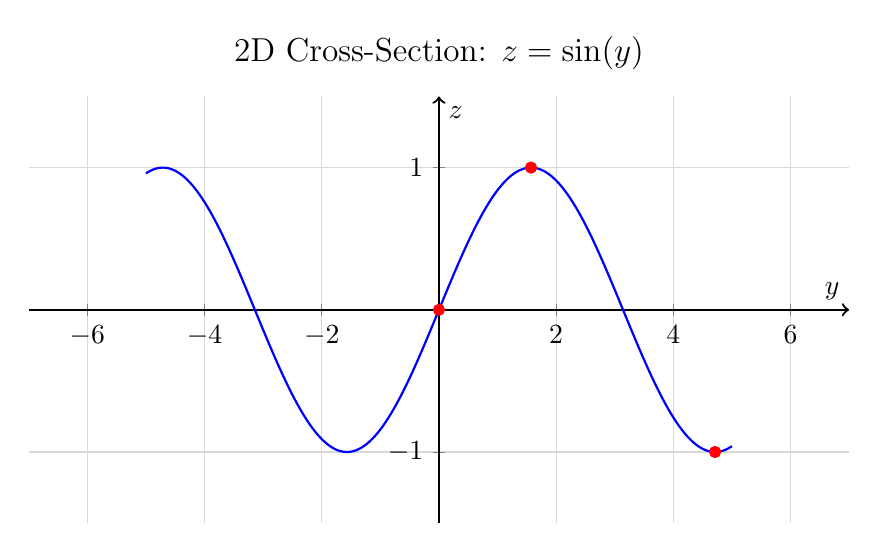
\begin{tikzpicture}
\begin{axis}[
    xlabel={$y$},
    ylabel={$z$},
    title={2D Cross-Section: $z = \sin(y)$},
    title style={font=\large},
    width=12cm,
    height=7cm,
    grid=major,
    grid style={gray!30},
    xmin=-7, xmax=7,
    ymin=-1.5, ymax=1.5,
    samples=200,
    axis lines=middle,
    axis line style={->, thick},
]
\addplot[blue, thick, smooth] {sin(deg(x))};
\addplot[red, only marks, mark=*] coordinates {(0,0) (1.5708,1) (4.7124,-1)};
\end{axis}
\end{tikzpicture}
\end{document}